\documentclass[aspectratio=169]{beamer}

\usetheme{Boadilla}
\usefonttheme{professionalfonts}
\setbeamertemplate{navigation symbols}{}
\setbeamertemplate{itemize items}[circle]
\setbeamertemplate{enumerate items}[default]
\setbeamertemplate{headline}{}

\usepackage[utf8]{inputenc}
\usepackage[T1]{fontenc}
\usepackage{lmodern}
\usepackage{amsmath}
\usepackage{booktabs}
\usepackage{tabularx}
\usepackage{array}
\usepackage{hyperref}
\usepackage[strings]{underscore}
\usepackage{listings}
\usepackage{tikz}
\usetikzlibrary{arrows.meta,positioning,fit,calc,shapes.geometric}
\usepackage{xcolor}

\definecolor{courseblue}{HTML}{12355B}
\definecolor{coursegold}{HTML}{C98A2E}
\definecolor{courseice}{HTML}{EEF3F8}
\definecolor{coursegreen}{HTML}{2F6B4F}
\definecolor{coursegray}{HTML}{4B5563}
\definecolor{codebg}{HTML}{F7F9FC}
\definecolor{codecomment}{HTML}{5E6C84}
\definecolor{codestring}{HTML}{0B6E4F}

\setbeamercolor{palette primary}{bg=courseblue,fg=white}
\setbeamercolor{palette secondary}{bg=coursegold,fg=white}
\setbeamercolor{palette tertiary}{bg=courseblue,fg=white}
\setbeamercolor{palette quaternary}{bg=coursegold,fg=white}
\setbeamercolor{structure}{fg=courseblue}
\setbeamercolor{frametitle}{bg=courseice,fg=courseblue}
\setbeamercolor{title}{fg=courseblue}
\setbeamercolor{block title}{bg=courseblue,fg=white}
\setbeamercolor{block body}{bg=courseice,fg=black}
\setbeamercolor{normal text}{fg=black,bg=white}
\setbeamercolor{alerted text}{fg=coursegold}

\setbeamerfont{footline}{size=\scriptsize}

\setbeamertemplate{footline}{
  \leavevmode
  \hbox{
    \begin{beamercolorbox}[wd=.33\paperwidth,ht=2.8ex,dp=1.2ex,leftskip=0.8em]{palette primary}%
      University of Trieste
    \end{beamercolorbox}%
    \begin{beamercolorbox}[wd=.49\paperwidth,ht=2.8ex,dp=1.2ex,center]{palette tertiary}%
      \coursename{} \textbar{} \coursecode
    \end{beamercolorbox}%
    \begin{beamercolorbox}[wd=.18\paperwidth,ht=2.8ex,dp=1.2ex,right,rightskip=0.8em]{palette secondary}%
      \insertframenumber{} / \inserttotalframenumber
    \end{beamercolorbox}%
  }
}

\hypersetup{
  colorlinks=true,
  linkcolor=courseblue,
  urlcolor=coursegreen
}

\lstdefinestyle{coursepython}{
  language=Python,
  basicstyle=\ttfamily\footnotesize,
  keywordstyle=\color{courseblue}\bfseries,
  commentstyle=\color{codecomment}\itshape,
  stringstyle=\color{codestring},
  showstringspaces=false,
  columns=fullflexible,
  keepspaces=true,
  frame=single,
  framerule=0.6pt,
  rulecolor=\color{courseblue},
  backgroundcolor=\color{codebg},
  xleftmargin=0.4em,
  xrightmargin=0.4em,
  aboveskip=0.4em,
  belowskip=0.2em
}

\newcommand{\coursename}{Data-driven Systems Engineering}
\newcommand{\coursecode}{440MI / 305SM}
\newcommand{\coursefooter}{}

\newcommand{\learninggoals}[1]{
  \begin{block}{Learning goals}
  #1
  \end{block}
}

\newcommand{\repoactivity}[1]{
  \begin{block}{Repo activity}
  #1
  \end{block}
}

\newcommand{\readinglist}[1]{
  \begin{block}{Papers and materials}
  {\footnotesize #1}
  \end{block}
}

\newcommand{\coursecontextframe}[5]{
  \begin{frame}{Course Map and Running Cases}
  \centering
  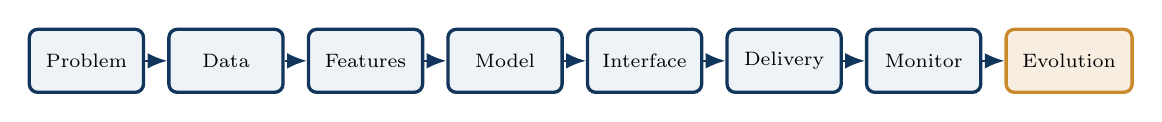
\begin{tikzpicture}[node distance=0.28cm]
  \node[flowbox, minimum width=1.45cm, minimum height=0.8cm] (problem) {\scriptsize Problem};
  \node[flowbox, minimum width=1.45cm, minimum height=0.8cm, right=of problem] (data) {\scriptsize Data};
  \node[flowbox, minimum width=1.45cm, minimum height=0.8cm, right=of data] (features) {\scriptsize Features};
  \node[flowbox, minimum width=1.45cm, minimum height=0.8cm, right=of features] (model) {\scriptsize Model};
  \node[flowbox, minimum width=1.45cm, minimum height=0.8cm, right=of model] (interface) {\scriptsize Interface};
  \node[flowbox, minimum width=1.45cm, minimum height=0.8cm, right=of interface] (delivery) {\scriptsize Delivery};
  \node[flowbox, minimum width=1.45cm, minimum height=0.8cm, right=of delivery] (monitor) {\scriptsize Monitor};
  \node[accentbox, minimum width=1.6cm, minimum height=0.8cm, right=of monitor] (evolution) {\scriptsize Evolution};
  \foreach \a/\b in {problem/data,data/features,features/model,model/interface,interface/delivery,delivery/monitor,monitor/evolution} {
    \draw[arrow] (\a) -- (\b);
  }
  \end{tikzpicture}

  \vspace{0.5em}
  \begin{block}{Today in the course}
  \textbf{Focus:} #1

  \textbf{Bridge:} #2
  \end{block}

  \begin{columns}[T]
  \column{0.48\textwidth}
  \begin{block}{Fraud case}
  {\footnotesize #3}
  \end{block}
  \column{0.48\textwidth}
  \begin{block}{Pasteurization case}
  {\footnotesize #4}
  \end{block}
  \end{columns}

  \vspace{0.3em}
  {\footnotesize \textbf{Course thread:} #5}
  \coursefooter
  \end{frame}
}

\newcommand{\classclosingframe}[4]{
  \begin{frame}{From This Class to the Next}
  \begin{block}{What stays with us}
  #1
  \end{block}

  \begin{columns}[T]
  \column{0.48\textwidth}
  \begin{block}{Project use}
  {\footnotesize #2}
  \end{block}
  \column{0.48\textwidth}
  \begin{block}{Next connection}
  {\footnotesize #3}
  \end{block}
  \end{columns}

  \vspace{0.3em}
  {\footnotesize \textbf{Course thread:} #4}
  \coursefooter
  \end{frame}
}

\tikzset{
  flowbox/.style={
    rounded corners=3pt,
    draw=courseblue,
    fill=courseice,
    very thick,
    minimum width=2.2cm,
    minimum height=0.9cm,
    align=center,
    font=\small
  },
  accentbox/.style={
    rounded corners=3pt,
    draw=coursegold,
    fill=coursegold!15,
    very thick,
    minimum width=2.2cm,
    minimum height=0.9cm,
    align=center,
    font=\small
  },
  arrow/.style={
    -{Latex[length=2.5mm,width=2mm]},
    thick,
    draw=courseblue
  }
}

\usepackage{amssymb}

\title{Class 20: Model Deployment and Prediction Serving}
\author{\coursename}
\date{}

\begin{document}

\frame{\titlepage \coursefooter}

\begin{frame}{Agenda}
\begin{itemize}
\item From a trained artifact to a callable, running service.
\item Flask as a service layer, Streamlit as a presentation layer.
\item The serving components of this repository, and what they lack.
\item Serving patterns and production concerns beyond a demonstration.
\item Closing the Data-Driven block and opening the MLOps block.
\end{itemize}
\coursefooter
\end{frame}

\begin{frame}{A model creates value only through an interface}
\begin{itemize}
\item A trained model that cannot be invoked or interpreted has limited practical value, regardless of its offline metrics.
\item An interface makes predictions available to users, services, and operational workflows.
\item A served model is a small software system with three parts: an interface, a preprocessing contract, and an operational surface (health, logs, versions).
\end{itemize}
\coursefooter
\end{frame}

\begin{frame}{Flask and Streamlit play different roles}
\begin{tabularx}{\textwidth}{>{\bfseries}l X}
Flask & A web framework for programmable endpoints over the Hypertext Transfer Protocol (HTTP), such as \texttt{POST /predict} or a streaming route. \\
\addlinespace[0.3em]
Streamlit & A framework for interactive user interfaces in Python: demonstrations, dashboards, exploratory tools. \\
\addlinespace[0.3em]
Combined & A common pattern: Flask as the back-end service, consumed by other programs, and Streamlit as the human-facing front end. \\
\bottomrule
\end{tabularx}
\coursefooter
\end{frame}

\begin{frame}{Serving components of this repository}
\centering
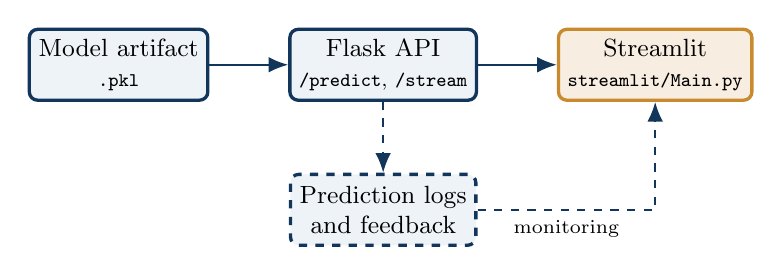
\begin{tikzpicture}[node distance=0.9cm and 1.0cm, font=\small]
\node[flowbox] (model) {Model artifact\\\scriptsize \texttt{.pkl}};
\node[flowbox, right=of model] (api) {Flask API\\\scriptsize \texttt{/predict}, \texttt{/stream}};
\node[accentbox, right=of api] (ui) {Streamlit\\\scriptsize \texttt{streamlit/Main.py}};
\node[flowbox, dashed, below=of api] (logs) {Prediction logs\\and feedback};
\draw[arrow] (model) -- (api);
\draw[arrow] (api) -- (ui);
\draw[arrow, dashed] (api) -- (logs);
\draw[arrow, dashed] (logs.east) -| node[pos=0.25, below, font=\scriptsize] {monitoring} (ui.south);
\end{tikzpicture}
\vspace{0.6em}
\begin{itemize}\footnotesize
\item Solid elements exist in the repository; dashed elements do not yet exist: no service records its predictions, so nothing can be monitored after deployment.
\item Closing this gap is the subject of continuous monitoring (Class 31).
\end{itemize}
\coursefooter
\end{frame}

\begin{frame}[fragile]{Repository example: the fraud scoring endpoint}
\begin{lstlisting}[style=coursepython]
model = pickle.load(open("notebooks/best_random_forest_model.pkl", "rb"))

@app.route("/")
def index():
    return jsonify({"message": "Model API running"}), 200

@app.route("/predict", methods=["POST"])
def predict():
    data = request.get_json(force=True)
    features = np.array(data["features"]).reshape(1, -1)
    pred = model.predict(features)[0]
    return jsonify({"prediction": int(pred)})
\end{lstlisting}
\begin{itemize}
\item This is the complete serving logic of \texttt{Class6\_model\_api.py}: load the model once at start-up and expose one prediction route.
\item It is intentionally minimal, so that what a service boundary contains, and what it still lacks, is visible.
\end{itemize}
\coursefooter
\end{frame}

\begin{frame}{What the minimal endpoint lacks}
\begin{itemize}
\item \textbf{A deployable artifact:} the file \texttt{notebooks/best\_random\_forest\_model.pkl} does not exist in the repository, so the service fails at start-up; the training notebook saves \texttt{model.pkl}.
\item \textbf{The preprocessing contract:} the model was trained on standardized features, but the endpoint passes raw features without the scaler. This \emph{training--serving skew}, $f(\mathbf{x}) \neq f(\phi_{\mathrm{train}}(\mathbf{x}))$, produces wrong predictions without any error message.
\item \textbf{Input validation:} \texttt{data["features"]} is trusted to contain exactly 30 numbers; any other request raises an unhandled exception.
\item \textbf{A useful response:} only a bare class $0/1$, without the probability, the threshold, or the model version.
\item \textbf{Operational surface:} no logging, and \texttt{debug=True} on \texttt{0.0.0.0} exposes the interactive debugger to the network, which allows remote code execution.
\end{itemize}
\coursefooter
\end{frame}

\begin{frame}{Training--serving skew, measured}
\begingroup\small
The deployed random forest (\texttt{streamlit/model.pkl}) applied to the 56{,}962 test transactions, with and without the scaler used in training ($\tau = 0.5$):
\par\endgroup
\vspace{0.5em}
\centering
\begingroup\footnotesize
\begin{tabular}{l c c c}
Input to the model & Frauds detected (TP) & Missed (FN) & False alarms (FP) \\
\toprule
Standardized, as in training & 81 & 17 & 5 \\
Raw features, as in \texttt{Class6\_model\_api.py} & 79 & 19 & 16 \\
\bottomrule
\end{tabular}
\par\endgroup
\vspace{0.6em}
\begin{itemize}\footnotesize
\item The service raises no error: it silently returns worse predictions, with three times as many false alarms.
\item The damage is moderate here because \texttt{V1}--\texttt{V28} are principal components whose scale is already close to unit variance; only \texttt{Time} and \texttt{Amount} change substantially. With features on very different scales, the degradation would be much larger.
\item Remedy: persist the preprocessing together with the model (or as one \texttt{Pipeline} object) and load both in the service.
\end{itemize}
\coursefooter
\end{frame}

\begin{frame}{A corrected service: \texttt{serving/fraud\_api.py}}
\begingroup\footnotesize
\renewcommand{\arraystretch}{1.25}
\begin{tabularx}{\textwidth}{>{\bfseries}l >{\raggedright\arraybackslash}X >{\raggedright\arraybackslash}X}
& \bfseries \texttt{Class6\_model\_api.py} & \bfseries \texttt{serving/fraud\_api.py} \\
\toprule
Artifact & Missing file; the service does not start & \texttt{streamlit/model.pkl}, identified by a hash (model version) \\
Preprocessing & None (training--serving skew) & The scaler fitted in training \\
Validation & None; malformed input raises an exception & 30 finite numbers, otherwise status 400 with a message \\
Response & Bare class $0/1$ & Probability, explicit threshold, decision, version, request identifier, latency \\
Logging & None & One JSON line per prediction (inputs and outputs) \\
Operations & \texttt{debug=True} on \texttt{0.0.0.0} & \texttt{GET /health}; debugger disabled; bound to localhost \\
\bottomrule
\end{tabularx}
\par\endgroup
\vspace{0.4em}
{\scriptsize The minimal file is kept unchanged in the repository as a teaching example. Run the corrected service from the repository root: \texttt{python serving/fraud\_api.py} (port 5001).\par}
\coursefooter
\end{frame}

\begin{frame}[fragile]{The corrected service: real responses}
\begin{columns}[T]
\column{0.53\textwidth}
\textbf{\footnotesize\texttt{POST /predict}, a fraudulent test transaction} {\scriptsize (200)}
\begin{lstlisting}[basicstyle=\ttfamily\scriptsize, columns=fullflexible, keepspaces=true, frame=single, backgroundcolor=\color{codebg}, rulecolor=\color{courseblue!40}]
{
  "fraud_probability": 0.915,
  "is_fraud": true,
  "threshold": 0.5,
  "model_version": "1382290f145e",
  "request_id": "f98e4f26-...",
  "latency_ms": 11.21
}
\end{lstlisting}
\column{0.43\textwidth}
\textbf{\footnotesize 29 values instead of 30} {\scriptsize (400)}
\begin{lstlisting}[basicstyle=\ttfamily\scriptsize, columns=fullflexible, keepspaces=true, frame=single, backgroundcolor=\color{codebg}, rulecolor=\color{courseblue!40}]
{"error": "\"features\" must be a
 list of 30 numbers (Time, V1,
 ..., Amount)"}
\end{lstlisting}
\textbf{\footnotesize A non-numeric value} {\scriptsize (400)}
\begin{lstlisting}[basicstyle=\ttfamily\scriptsize, columns=fullflexible, keepspaces=true, frame=single, backgroundcolor=\color{codebg}, rulecolor=\color{courseblue!40}]
{"error": "\"features\" must contain
 only finite numbers"}
\end{lstlisting}
\end{columns}
\vspace{0.3em}
\begin{itemize}\footnotesize
\item A legitimate transaction from the same test split receives a probability of 0.005. Every response is also appended to \texttt{logs/predictions.jsonl}, which is excluded from Git.
\end{itemize}
\coursefooter
\end{frame}

\begin{frame}{Repository example: the dashboard hub}
\centering
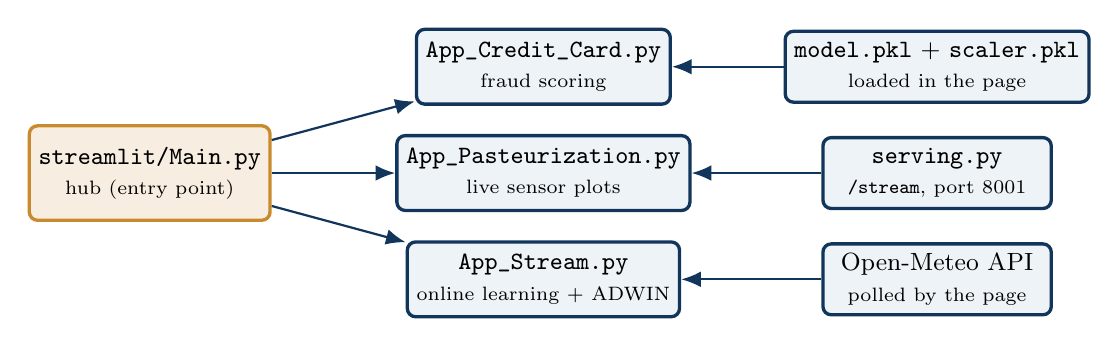
\begin{tikzpicture}[font=\footnotesize, box/.style={flowbox, minimum width=3.2cm, minimum height=0.95cm}]
\node[accentbox, minimum width=2.6cm, minimum height=1.2cm] (hub) at (0,0) {\texttt{streamlit/Main.py}\\\scriptsize hub (entry point)};
\node[box] (cc) at (5.0,1.35) {\texttt{App\_Credit\_Card.py}\\\scriptsize fraud scoring};
\node[box] (pa) at (5.0,0) {\texttt{App\_Pasteurization.py}\\\scriptsize live sensor plots};
\node[box] (as) at (5.0,-1.35) {\texttt{App\_Stream.py}\\\scriptsize online learning + ADWIN};
\node[flowbox, minimum width=2.9cm] (s1) at (10.0,1.35) {\texttt{model.pkl} + \texttt{scaler.pkl}\\\scriptsize loaded in the page};
\node[flowbox, minimum width=2.9cm] (s2) at (10.0,0) {\texttt{serving.py}\\\scriptsize \texttt{/stream}, port 8001};
\node[flowbox, minimum width=2.9cm] (s3) at (10.0,-1.35) {Open-Meteo API\\\scriptsize polled by the page};
\draw[arrow] (hub) -- (cc); \draw[arrow] (hub) -- (pa); \draw[arrow] (hub) -- (as);
\draw[arrow] (s1) -- (cc); \draw[arrow] (s2) -- (pa); \draw[arrow] (s3) -- (as);
\end{tikzpicture}
\vspace{0.6em}
\begin{itemize}\footnotesize
\item \texttt{streamlit run streamlit/Main.py} starts the hub; Streamlit discovers every file in \texttt{pages/} and lists it in the navigation.
\item The three pages use three different serving patterns: a model loaded inside the user interface, a separate streaming service, and an external application programming interface (API).
\end{itemize}
\coursefooter
\end{frame}

\begin{frame}{Serving patterns}
\begin{tabularx}{\textwidth}{>{\bfseries}l X}
Batch scoring & Predictions are computed periodically for a stored dataset and stored for later use; latency is irrelevant, throughput matters. \\
\addlinespace[0.3em]
Online request--response & A client sends one request and waits synchronously for one prediction, as in \texttt{Class6\_model\_api.py}; latency is critical. \\
\addlinespace[0.3em]
Streaming & Predictions are computed continuously over an incoming event stream, as in the pasteurization case (Classes 18--19). \\
\bottomrule
\end{tabularx}
\coursefooter
\end{frame}

\begin{frame}{Production concerns not covered by the demonstrations}
\begin{itemize}\small
\item \textbf{Performance:} latency budgets and load tests. Measured on 1{,}000 sequential requests to \texttt{serving/fraud\_api.py}: 50th percentile 14\,ms, 95th percentile 17.5\,ms. With the random forest as trained (\texttt{n\_jobs=-1}), the same requests took 41 and 86\,ms: parallelism designed for training slows down single predictions.
\item \textbf{Serving infrastructure:} Flask itself warns that its development server must not be used in production; a production deployment uses a Web Server Gateway Interface (WSGI) server (e.g.\ Gunicorn) behind a reverse proxy.
\item \textbf{Versioning and compatibility:} \texttt{model.pkl} was serialized with scikit-learn 1.7.2, whereas \texttt{requirements.txt} pins 1.6.0; a model registry stores the artifact with the exact library versions needed to load it.
\item \textbf{Observability:} structured logs (now present), request tracing, and alerts on error rates.
\end{itemize}
\coursefooter
\end{frame}

\begin{frame}{From a demonstration service to a production deployment}
\centering
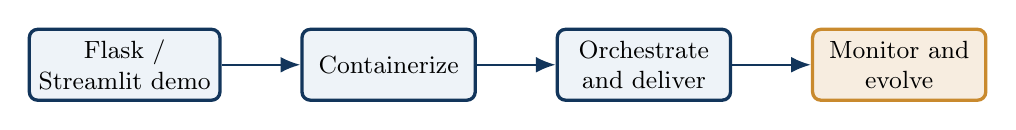
\begin{tikzpicture}[node distance=1cm and 1cm]
\node[flowbox] (demo) {Flask /\\Streamlit demo};
\node[flowbox, right=of demo] (container) {Containerize};
\node[flowbox, right=of container] (orchestrate) {Orchestrate\\and deliver};
\node[accentbox, right=of orchestrate] (monitor) {Monitor and\\evolve};
\draw[arrow] (demo) -- (container);
\draw[arrow] (container) -- (orchestrate);
\draw[arrow] (orchestrate) -- (monitor);
\end{tikzpicture}
\vspace{0.6em}
\begin{itemize}
\item Each step is developed in the MLOps block: containers and continuous integration and delivery (CI/CD) in Class 30, monitoring and scalability in Class 31.
\end{itemize}
\coursefooter
\end{frame}

\begin{frame}{Repository connections}
\repoactivity{
\begin{itemize}
\item \texttt{Class6\_model\_api.py}: the minimal Flask serving example for the fraud case; \texttt{serving/fraud\_api.py}: its corrected counterpart.
\item \texttt{streamlit/Main.py}: the hub that presents the fraud, pasteurization, and online-learning pages together.
\item \texttt{pasteurization/serving.py}: the same serving concerns applied to a continuous stream instead of single requests.
\end{itemize}
}
\coursefooter
\end{frame}

\begin{frame}{Readiness checklist before calling a model ``served''}
\begin{itemize}
\item Does the service start from a clean checkout of the repository, with the referenced artifacts present?
\item Can it reject a malformed request with an informative error instead of crashing?
\item Is the preprocessing at inference identical to the preprocessing used in training?
\item Is it recorded which model version answered each request?
\item Could a teammate other than the author redeploy the service from its documentation?
\end{itemize}
\coursefooter
\end{frame}

\begin{frame}{Papers and materials}
\readinglist{
\fontsize{6.8}{8.2}\selectfont
\begin{columns}[T]
\column{0.5\textwidth}
\begin{itemize}\setlength{\itemsep}{1pt}
\item Sculley, D., Holt, G., Golovin, D., Davydov, E., Phillips, T., Ebner, D., Chaudhary, V., Young, M., Crespo, J.-F., Dennison, D. (2015). Hidden technical debt in machine learning systems. \emph{Advances in Neural Information Processing Systems}, 28, 2503--2511.
\item Breck, E., Cai, S., Nielsen, E., Salib, M., Sculley, D. (2017). The ML test score: A rubric for ML production readiness and technical debt reduction. \emph{Proceedings of the IEEE International Conference on Big Data}, 1123--1132.
\item Paleyes, A., Urma, R.-G., Lawrence, N.\,D. (2022). Challenges in deploying machine learning: A survey of case studies. \emph{ACM Computing Surveys}, 55(6), 114:1--114:29.
\end{itemize}
\column{0.5\textwidth}
\begin{itemize}\setlength{\itemsep}{1pt}
\item Gift, N., Deza, A. (2021). \emph{Practical MLOps}. O'Reilly.
\item Wiggins, A. (2017). \href{https://12factor.net/}{The Twelve-Factor App}.
\item Documentation: \href{https://flask.palletsprojects.com/en/stable/}{Flask}; \href{https://docs.streamlit.io/}{Streamlit}.
\end{itemize}
\end{columns}
}
\coursefooter
\end{frame}

\begin{frame}{Take-away message}
\vfill
\centering
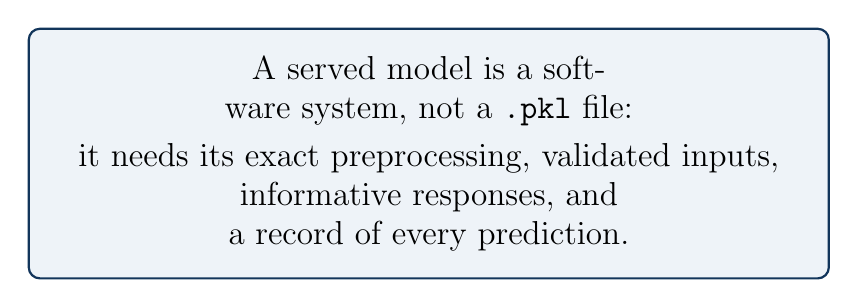
\begin{tikzpicture}
\node[fill=courseice, draw=courseblue, thick, rounded corners=4pt, inner sep=10pt, text width=0.78\textwidth, align=center, font=\large] {A served model is a software system, not a \texttt{.pkl} file:\\[0.3em] it needs its exact preprocessing, validated inputs,\\ informative responses, and a record of every prediction.};
\end{tikzpicture}

\vfill
{\Large\bfseries\color{courseblue} Thank you for your attention.}

\vspace{0.4em}
{\small\color{coursegray} This concludes the Data-Driven block. Next: Class 21 --- Cybertec (invited talk), opening the MLOps block.}
\vfill
\coursefooter
\end{frame}

\end{document}
